\documentclass{beamer}
\usepackage[utf8]{inputenc}
\usepackage{tikz} % For semi-transparent background blocks
\usepackage{hyperref}
\usepackage{multimedia}
\usepackage{ulem}
\usepackage{wasysym}

\usepackage{pbox}

%%%%%%%%%%%%%%%%%%%%%%%%%%%%%%%%%%%%%%%%%%%%%%%%%%%%%%%%%%%%%%%%%%%
% Style modifications
%%%%%%%%%%%%%%%%%%%%%%%%%%%%%%%%%%%%%%%%%%%%%%%%%%%%%%%%%%%%%%%%%%%

\usetheme{Berlin}

%%% Fonts %%%

% Change font. Fontspec requires xelatex instead of pdflatex!
% Font catalog: http://www.tug.dk/FontCatalogue/
\usepackage{fontspec}

%\setsansfont{Comfortaa}
%\setsansfont{DejaVu Sans}
%\setsansfont{Fira Sans}

% Use "Fira Sans Light" as the normal font and the "Fira Sans" for
% bold fonts
\setsansfont[
  ItalicFont={Fira Sans Light Italic},
  BoldFont={Fira Sans},
  BoldItalicFont={Fira Sans Italic}]{Fira Sans Light}

\setbeamerfont{title}{size=\huge, series=\bfseries}
\setbeamerfont{frametitle}{size=\large, series=\bfseries}
\setbeamerfont{block body}{size=\huge}

%%% Slide template %%%

\setbeamertemplate{frames}[default]

% Empty headline / footline
\setbeamertemplate{headline}{}
\setbeamertemplate{footline}{}

% Remove navigation icons
\setbeamertemplate{navigation symbols}{}

%%% Colors %%%

\usecolortheme{crane}

\definecolor{lightgray}{RGB}{245,245,245}
\definecolor{darkgray}{RGB}{45,45,45}

% Use the slide background in block environments                                                                                                      

\setbeamercolor{title}{fg=white,bg=darkgray}

\setbeamertemplate{blocks}[default]
\setbeamercolor{block title}{bg=}
\setbeamercolor{block body}{bg=lightgray}
\setbeamercolor{frametitle}{fg=white,bg=darkgray}
\setbeamercolor{itemize item}{fg=darkgray}
\setbeamertemplate{itemize items}[circle]
\setbeamercolor{section number projected}{bg=darkgray,fg=white}
\setbeamercolor{section in toc}{fg=darkgray}
\setbeamercolor{subsection in toc}{fg=darkgray}

\addtobeamertemplate{block begin}{\pgfsetfillopacity{0.8}}{\pgfsetfillopacity{1}}
\addtobeamertemplate{frametitle}{\pgfsetfillopacity{0.8}}{\pgfsetfillopacity{1}}
\addtobeamertemplate{title page}{\pgfsetfillopacity{0.8}}{\pgfsetfillopacity{1}}

%%% Misc %%%

% Command to place the test (e.g. citation) in the center of the footer
\newcommand{\setfootercentertext}[1]{
\setbeamertemplate{footline}{
  \hspace*{\fill}
  \raisebox{3mm}[0mm][0mm]{
    \tiny{#1}}\hspace*{\fill}}
}

%%%%%%%%%%%%%%%%%%%%%%%%%%%%%%%%%%%%%%%%%%%%%%%%%%%%%%%%%%%%%%%%%%%
% Content
%%%%%%%%%%%%%%%%%%%%%%%%%%%%%%%%%%%%%%%%%%%%%%%%%%%%%%%%%%%%%%%%%%%

%------------------------------------------------------------------------------
\title{What is good scientific practice\\for research software?}
%------------------------------------------------------------------------------

%\subtitle{Working Group Research Software}

\author{\small Konrad U. Förstner\\
  \vspace{0.5cm}
  \textcolor{orange}{@konradfoerstner}}

\institute{University of Würzburg}

\date{\scriptsize May 10$^{th}$, 2017}

\logo{
  \href{https://creativecommons.org/licenses/by/4.0/}{
    
\includegraphics[width=0.88cm]{images/creative_commons_attribute.png}}}
\begin{document}
\begin{frame}{}
  \titlepage
\end{frame}
\logo{}

\setbeamertemplate{background}{}


% Symbiosis of technology and science
% Tools - Science
% examples: Telescope / Microscope
\begin{frame}
  \frametitle{}
  \begin{block}{}
    \begin{center}
      Science $\rightleftarrows$ Technology
      \end{center}
  \end{block}
\end{frame}

% Telescope
\setbeamertemplate{background}{
  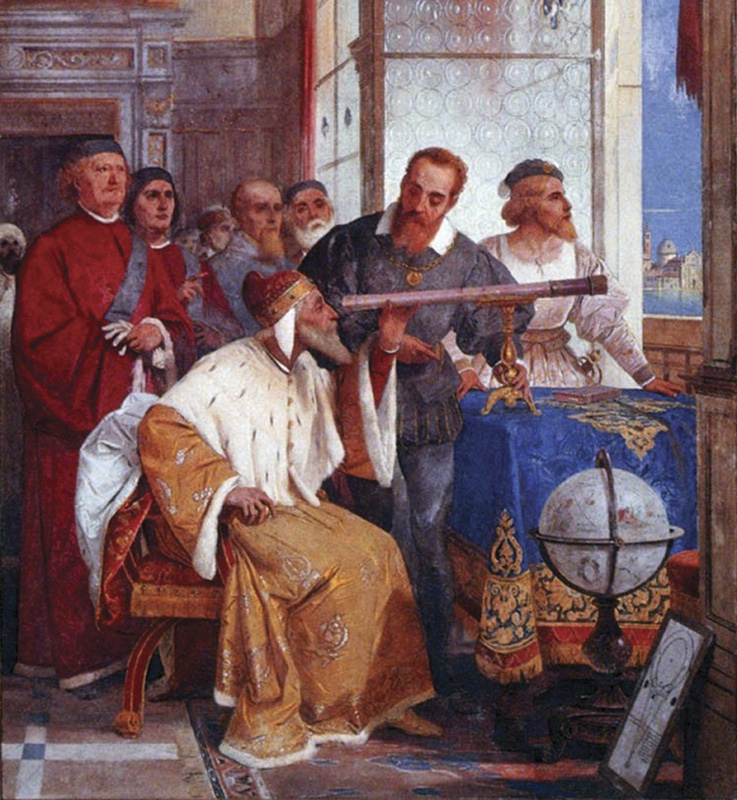
\includegraphics[width=\paperwidth]{images/Bertini_fresco_of_Galileo_Galilei_and_Doge_of_Venice.jpg}}
\setbeamertemplate{footline}{\raisebox{2mm}[2mm][2mm]{\Tiny{
      \href{https://commons.wikimedia.org/wiki/File:Bertini_fresco_of_Galileo_Galilei_and_Doge_of_Venice.jpg}{
        https://commons.wikimedia.org/wiki/File:Bertini\_fresco\_of\_Galileo\_Galilei\_and\_Doge\_of\_Venice.jpg} - PD}}}
\begin{frame}
\end{frame}

% Microscope
\setbeamertemplate{background}{
  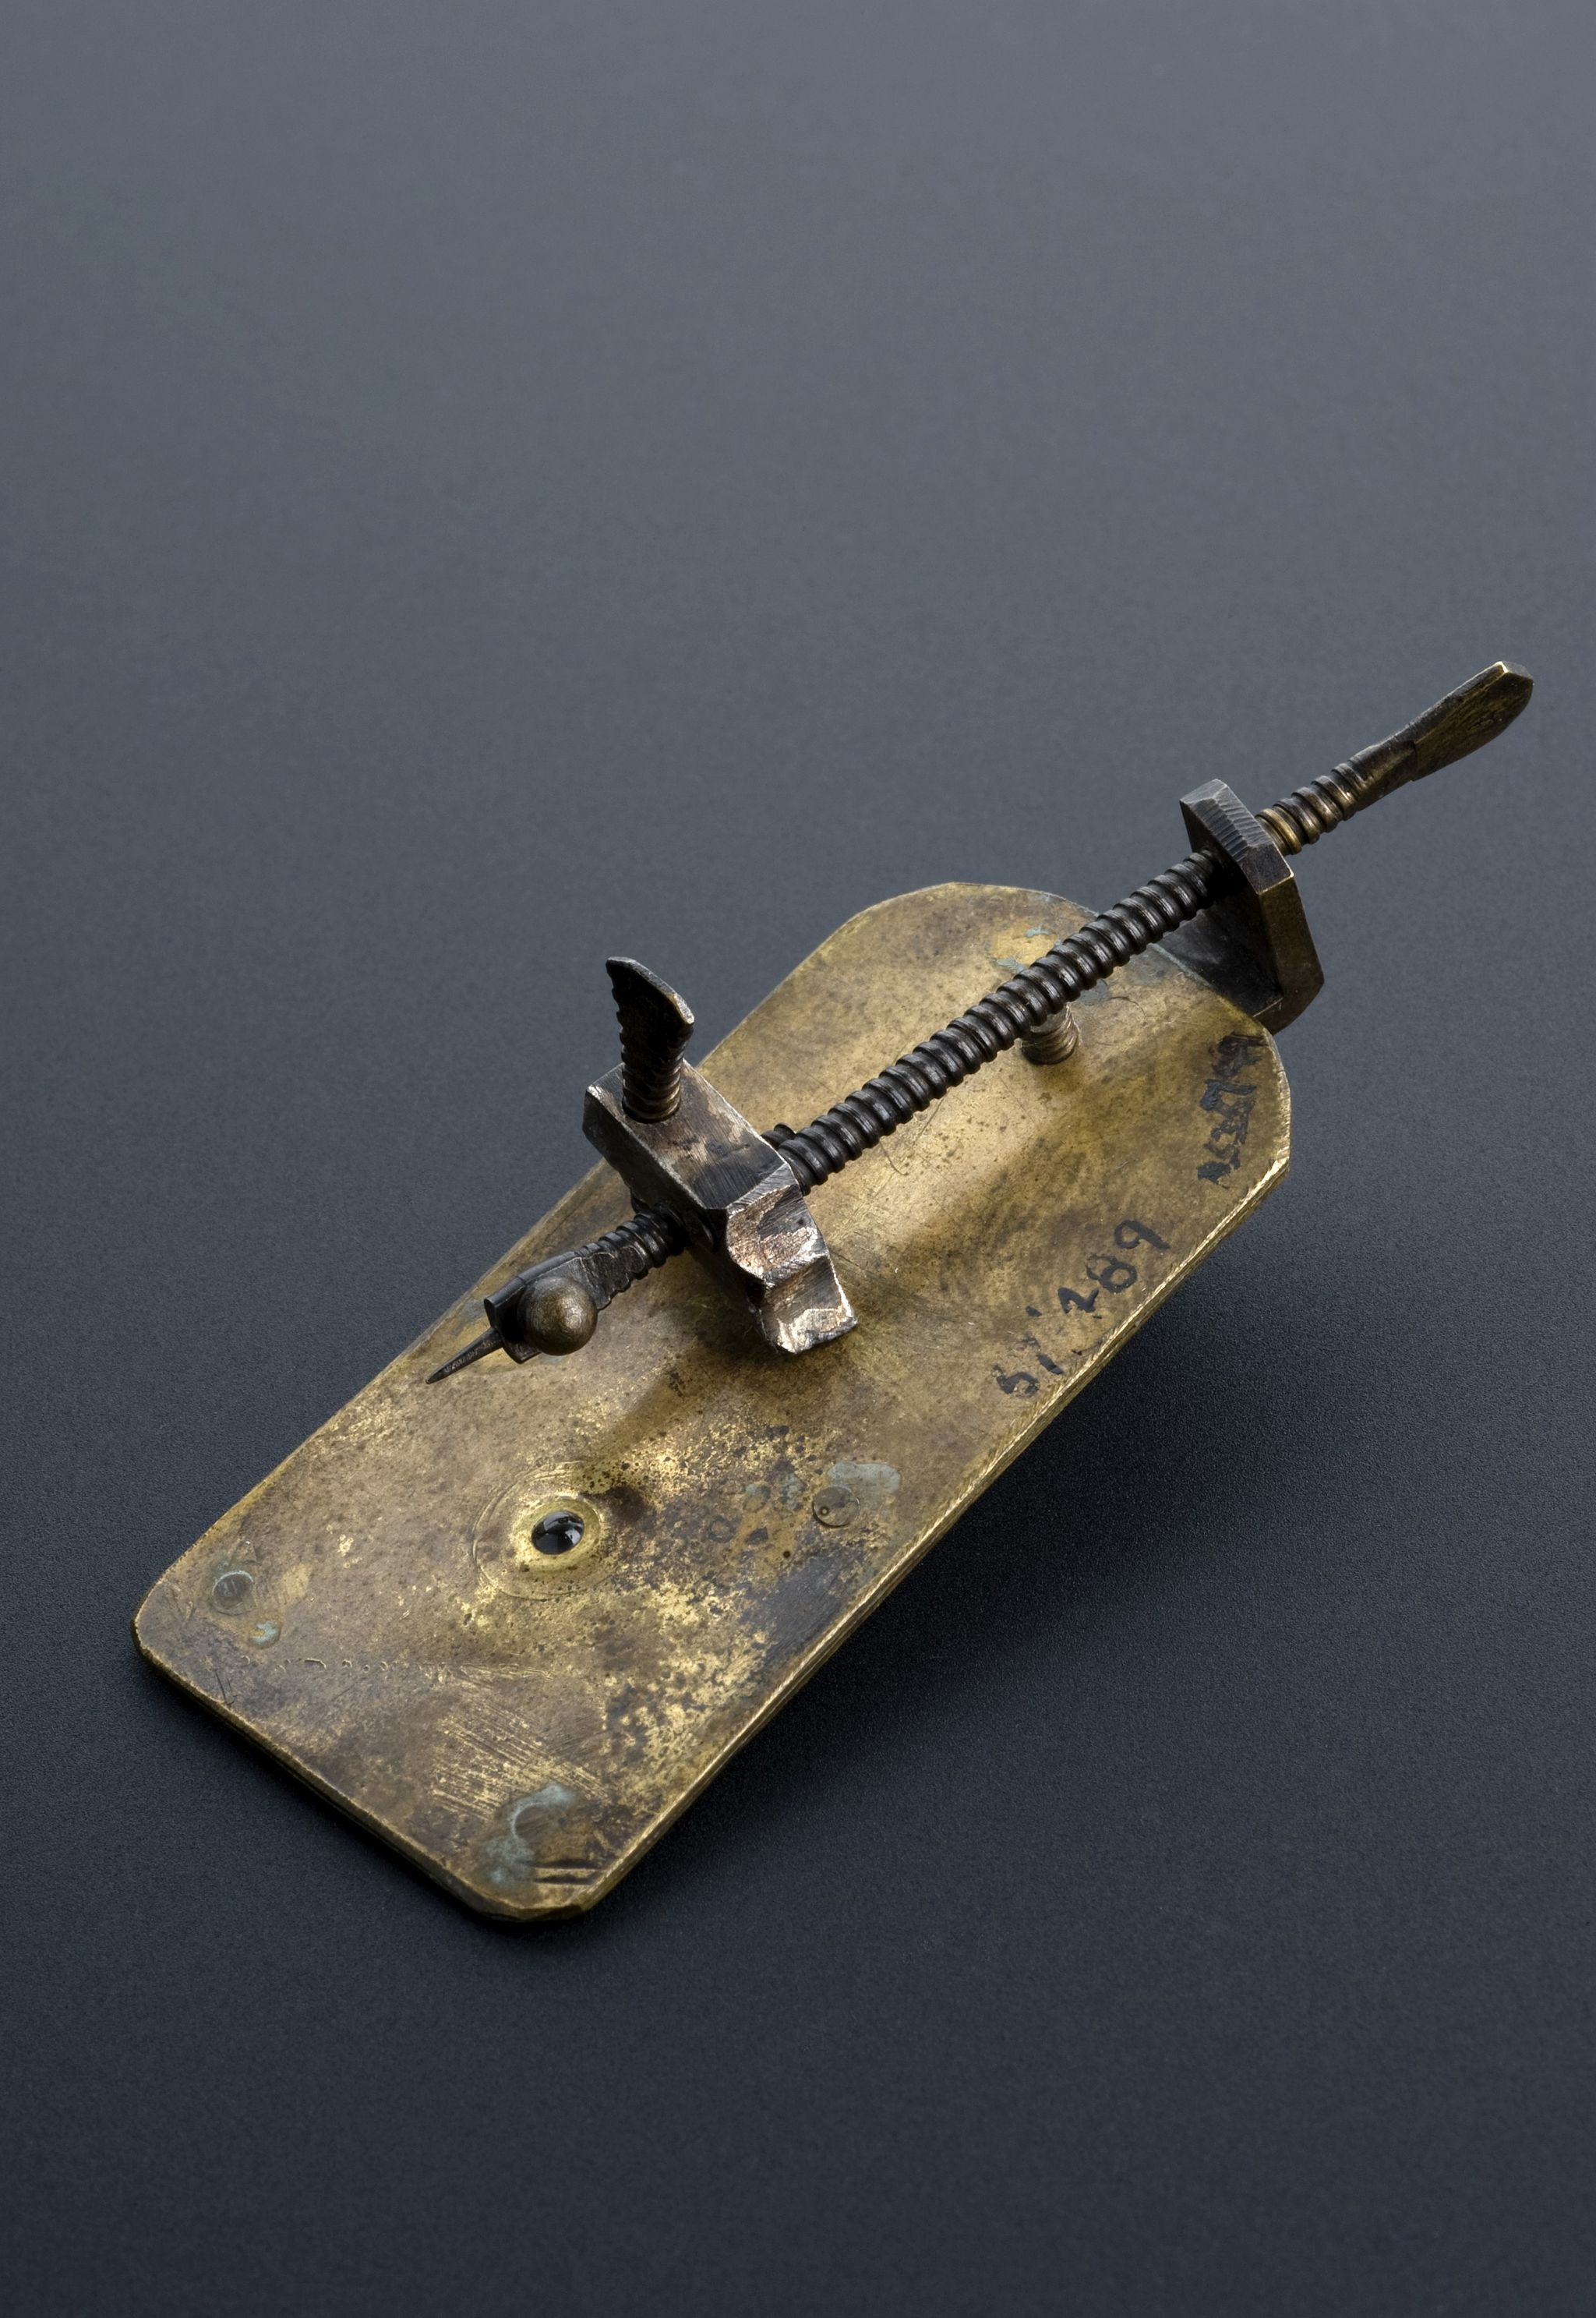
\includegraphics[width=\paperwidth,trim=0 0 0 210,clip]{images/2048px-Leeuwenhoek_simple_microscope_(copy),_Leyden,_1901-1930_Wellcome_L0057739.jpg}}
\setbeamertemplate{footline}{\raisebox{2mm}[2mm][2mm]{\Tiny{
      \href{https://commons.wikimedia.org/wiki/File:Leeuwenhoek_simple_microscope_(copy),_Leyden,_1901-1930_Wellcome_L0057739.jpg}{
        https://commons.wikimedia.org/wiki/File:Leeuwenhoek\_simple\_microscope\_(copy),\_Leyden,\_1901-1930\_Wellcome\_L0057739.jpg}
      - CC-By by Wiki Commons User \href{https://commons.wikimedia.org/wiki/User:Fae}{Fae}}}}
\begin{frame}
\end{frame}

\setbeamertemplate{background}{}
\setbeamertemplate{footline}{}

\begin{frame}
  \frametitle{}
  \begin{block}{}
    \begin{center}
      Thank you
      \end{center}    
  \end{block}
\end{frame}

\end{document}
